\section{Experiments}
\label{sec:experiments}

This section reports the experimental results of NTD-PL on synthetic data and real hyperspectral data under a unified protocol. The experiments proceed through shared settings, controlled synthetic data, and reconstruction and completion on real hyperspectral data, with the goal of clarifying the scope of applicability of the method, the source of its gains, and its computational cost.

\subsection{Experimental Setup}
\label{sec:exp-setup}

This subsection gives the data-generation principles, comparison protocol, and evaluation metrics shared by the subsequent experiments. Except for implementation details specific to individual subsections, all results follow the same reproducible experimental protocol.

To define nonlinear strength consistently across different nonlinear mappings, we define $\alpha$ as the energy ratio of the orthogonal nonlinear residual, rather than as the amplitude coefficient placed directly in front of the nonlinear function. Let the linear low-rank backbone be
\begin{equation}
\mathcal S^\star \in \mathbb R^{I_1\times \cdots \times I_N},
\end{equation}
and given an element-wise mapping $g(\cdot)$, we first construct the orthogonal residual relative to $\mathcal S^\star$:
\begin{equation}
\mathcal R^\star
=
g(\mathcal S^\star)
-
\frac{\langle g(\mathcal S^\star), \mathcal S^\star\rangle}{\|\mathcal S^\star\|_F^2}\,\mathcal S^\star,
\end{equation}
and then normalize it as
\begin{equation}
\widetilde{\mathcal R}^\star
=
\frac{\|\mathcal S^\star\|_F}{\|\mathcal R^\star\|_F}\,\mathcal R^\star.
\end{equation}
The final observation tensor is defined by
\begin{equation}
\mathcal Y_\alpha
=
\sqrt{1-\alpha}\,\mathcal S^\star
+
\sqrt{\alpha}\,\widetilde{\mathcal R}^\star,
\qquad 0\le \alpha\le 1.
\label{eq:exp-alpha-energy}
\end{equation}
Thus, $\alpha$ represents the proportion of observation energy allocated to the orthogonal nonlinear residual. As $\alpha$ increases, the observation progressively deviates from the linear low-rank backbone, rather than merely increasing in amplitude. The \texttt{affine shift control} appearing in the linear-consistency subsection is essentially the addition of a constant bias to linear Tucker source data followed by energy normalization.

The controlled synthetic experiments consider two polynomial residual families and two smooth residual families:
\begin{equation}
g_{\mathrm{poly2}}(s)=s^2,\qquad
g_{\mathrm{poly3}}(s)=s^2+s^3,
\end{equation}
\begin{equation}
g_{\sin}(s)=\sin(\kappa_{\sin}s),\qquad
g_{\tanh}(s)=\tanh(\kappa_{\tanh}s).
\end{equation}
Here, $\kappa_{\sin}$ and $\kappa_{\tanh}$ are set adaptively according to the input scale so that the functions do not stay in the linear regime for too long or saturate too early.

NMSE and RMSE are used as the main metrics. In the real hyperspectral experiments, full-observation reconstruction is uniformly reported using RMSE, NMSE, and SAM, while random-missing completion is primarily reported using RMSE$^\ast$, NMSE$^\ast$, and SAM$^\ast$. Metrics marked with $^\ast$ are computed only on genuinely missing entries and therefore serve as the primary indicators of completion quality.

For the percentage contribution of the $\beta_p$ terms discussed later, we uniformly use
\begin{equation}
c_p
=
\frac{\|\beta_p \mathcal S^{\odot p}\|_F}{\sum_{q=0}^{P}\|\beta_q \mathcal S^{\odot q}\|_F}\times 100\%.
\label{eq:beta-contribution}
\end{equation}
This definition characterizes the relative strength allocation of the terms of different orders in the overall expansion, and the values $\{c_p\}$ sum to exactly $100\%$ over $p$.

The linear low-rank baselines compared in this paper include Tucker, CP, TT, and TR. Tucker decomposition is the most direct linear reference for our method. CP decomposition represents a tensor as a sum of rank-one tensors; it has a more compact parameterization and is also one of the most classical baselines in low-rank tensor modeling \cite{Kolda2009Tensor}. TT decomposition uses a chain-structured core factorization for high-order tensors and can significantly reduce storage and computational cost in high-order settings \cite{oseledets2011}. TR decomposition further closes the chain structure into a ring, making rank allocation more flexible than in TT \cite{zhao2016tr}. Note that these decompositions differ in structure, and their notions of rank are not the same, so exact parameter matching is impossible. In the experiments, we choose ranks so that the parameter counts are as similar as possible.

\subsection{Controlled Synthetic Data Experiments}
\label{sec:exp-syn}

This subsection compares linear baselines and NTD-PL under controlled mechanisms. The experiments contain two parts: first, on linear source data, we compare the paired errors of Tucker and linearly restricted NTD-PL; second, under a unified nonlinear residual protocol, we compare how the errors of different methods vary with $\alpha$ and $P$.

\subsubsection{Linear-Consistency Verification}
\label{sec:linear-consistency}

On linear source data, we compare the paired errors of Tucker and NTD-PL to check whether the latter reduces exactly to Tucker. Specifically, the data are Tucker tensors generated under multiple random seeds, with rank $[4,4,4]$, together with an affine bias \texttt{bias}, followed by energy normalization and additive noise at $30$ dB. For NTD-PL, we set $P=6$ and optionally allow or disallow $\beta_0$.

Table~\ref{tab:linear-consistency} shows that when \texttt{bias=0}, the fitting errors of Tucker and NTD-PL without a constant term almost completely overlap, and the higher-order contributions are very small, confirming the linear consistency of NTD-PL. When \texttt{bias=0.5}, NTD-PL can still fit the data well, whereas Tucker and NTD-PL with restricted $\beta_0$ exhibit systematic bias. Interestingly, one can observe that when $\beta_0$ is restricted, NTD-PL automatically uses higher-order terms to fit the bias, and the result is still slightly better than Tucker. Further, the distribution of paired differences is shown in Appendix Figure~\ref{fig:linear-consistency-paired-gap}, where it is even more visually clear that when no affine bias is present, the difference between Tucker and NTD-PL is concentrated around zero, whereas in the presence of bias a more obvious systematic paired gap appears between the restricted model and Tucker.

\begin{table}[htbp]
    \centering
    \caption{Comparison of Tucker and NTD-PL on purely linear source data, used to verify the linear consistency of NTD-PL.}
    \label{tab:linear-consistency}
    \small
    \resizebox{\linewidth}{!}{%
    \begin{tabular}{c|c|c|c|c}
    \hline
    Setting & Method & RMSE & NMSE(dB) & $p>1$ contrib. (\%) \\
    \hline
    \multirow{3}{*}{bias=0} & Tucker & 0.011398 $\pm$ 0.000747 & -38.8822 $\pm$ 0.5704 & --- \\
     & NTD-PL ($\beta_0 = 0$) & 0.011610 $\pm$ 0.000658 & -38.7173 $\pm$ 0.4883 & 4.19 $\pm$ 2.80 \\
     & NTD-PL ($\beta_0$ free) & 0.011698 $\pm$ 0.000634 & -38.6500 $\pm$ 0.4650 & 3.19 $\pm$ 2.15 \\
    \hline
    \multirow{3}{*}{bias=0.5} & Tucker & 0.064650 $\pm$ 0.016502 & -24.0505 $\pm$ 2.0996 & --- \\
     & NTD-PL ($\beta_0 = 0$) & 0.052204 $\pm$ 0.011788 & -25.8466 $\pm$ 1.8304 & 39.17 $\pm$ 11.56 \\
     & NTD-PL ($\beta_0$ free) & 0.011797 $\pm$ 0.000596 & -38.5755 $\pm$ 0.4319 & 2.98 $\pm$ 2.00 \\
    \hline
\end{tabular}
}
\end{table}

\subsubsection{Experiments on Nonlinear Mapping Matching and Approximation}
\label{sec:nonlinearapprox}

Under the unified nonlinear generation protocol described in Section~\ref{sec:exp-setup}, we consider both polynomial and general nonlinear cases. Specifically, starting from Tucker tensors generated under multiple random seeds, we apply four classes of element-wise nonlinear residuals, namely \texttt{poly2}, \texttt{poly3}, \texttt{sin}, and \texttt{tanh}, and control the energy ratio of the nonlinear residual by \eqref{eq:exp-alpha-energy}. The experiment uniformly scans $\alpha\in\{0.10,0.15,0.20,0.25,0.30,0.35,0.40\}$ and $P\in\{1,2,3,4,5,6\}$, and compares the NMSE performance of Tucker, CP, TT, TR, and NTD-PL over $10$ random seeds under similar parameter budgets.

Figure~\ref{fig:nonlinear-alpha-grid} shows that under all types of nonlinear residuals, NTD-PL maintains a stable lead over the entire range of nonlinear strength, indicating its advantage in handling nonlinear residuals. In addition, the approximation error of NTD-PL can be seen to scale with $\alpha$, and the trend is consistent with the appendix discussion on the relation between truncation error and $\alpha$: under the generation protocol used in this paper, the greater the energy proportion of the nonlinear residual, the larger the orthogonal residual that a finite-order polynomial link needs to absorb. Therefore, the error curve rises overall as $\alpha$ increases, but the advantage of NTD-PL relative to linear baselines is retained.

\begin{figure}[htbp]
    \centering
    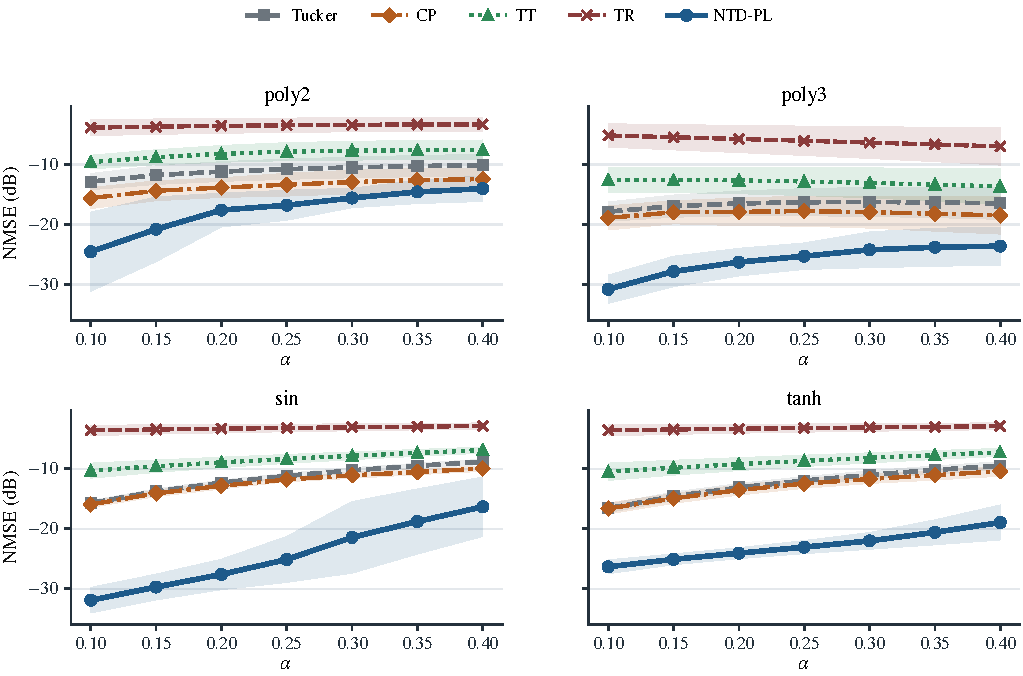
\includegraphics[width=\textwidth]{./inputs/figures/main/nonlinear_alpha_grid.pdf}
    \caption{Approximation error of NTD-PL and the baseline methods as a function of nonlinear strength.}
    \label{fig:nonlinear-alpha-grid}
\end{figure}

\begin{table}[htbp]
    \centering
    \caption{Contribution of each degree term in NTD-PL (in \%).}
    \label{tab:beta-contrib-nonlinear}
    \small
    \resizebox{\linewidth}{!}{%
    \begin{tabular}{c|c|c|c|c|c|c|c}
    \hline
    nonlinear($\alpha=0.25$) & $\beta_0$ & $\beta_1$ & $\beta_2$ & $\beta_3$ & $\beta_4$ & $\beta_5$ & $\beta_6$ \\
    \hline
    poly2 & 0.5 $\pm$ 0.8 & 43.3 $\pm$ 17.5 & 23.2 $\pm$ 6.9 & 5.8 $\pm$ 4.9 & 8.2 $\pm$ 5.8 & 9.1 $\pm$ 9.5 & 9.8 $\pm$ 9.7 \\
    poly3 & 0.1 $\pm$ 0.1 & 24.1 $\pm$ 6.5 & 9.8 $\pm$ 4.1 & 38.1 $\pm$ 9.0 & 7.3 $\pm$ 5.5 & 11.5 $\pm$ 11.1 & 9.1 $\pm$ 6.3 \\
    sin & 0.1 $\pm$ 0.1 & 37.7 $\pm$ 8.8 & 0.6 $\pm$ 0.6 & 35.4 $\pm$ 3.5 & 2.8 $\pm$ 2.7 & 19.8 $\pm$ 6.9 & 3.6 $\pm$ 3.8 \\
    tanh & 0.2 $\pm$ 0.1 & 37.9 $\pm$ 9.0 & 1.3 $\pm$ 0.7 & 30.9 $\pm$ 4.0 & 5.4 $\pm$ 3.7 & 17.3 $\pm$ 3.5 & 7.0 $\pm$ 5.8 \\
    \hline
\end{tabular}
}
\end{table}

\begin{figure}[htbp]
    \centering
    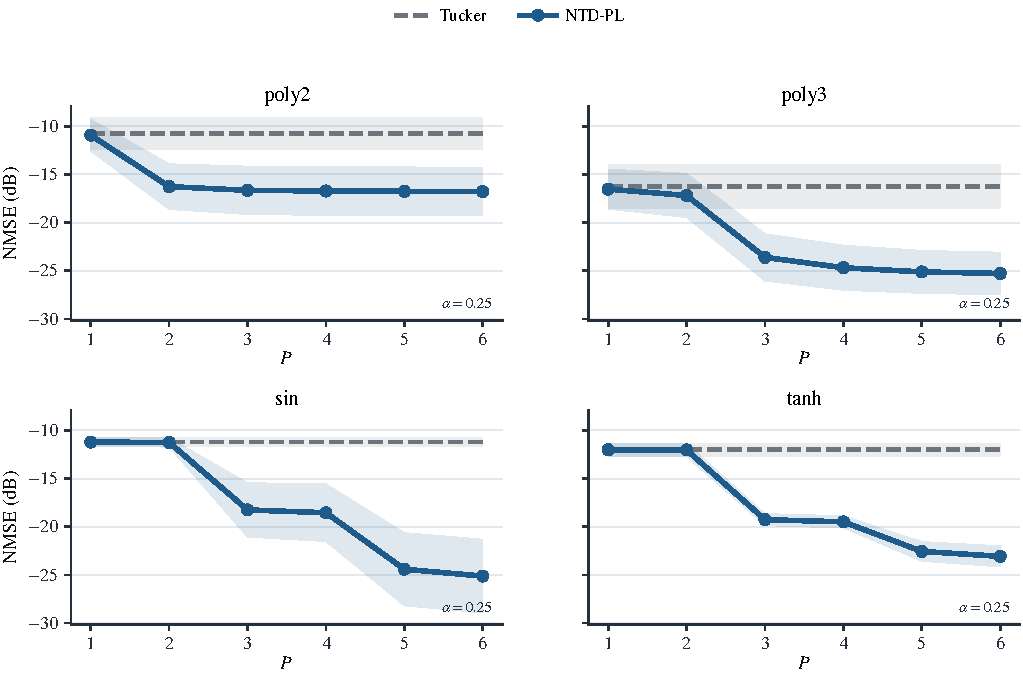
\includegraphics[width=\textwidth]{./inputs/figures/main/nonlinear_pmax_grid.pdf}
    \caption{Approximation error of NTD-PL as a function of the degree $P$.}
    \label{fig:nonlinear-pmax-grid}
\end{figure}

\begin{figure}[htbp]
    \centering
    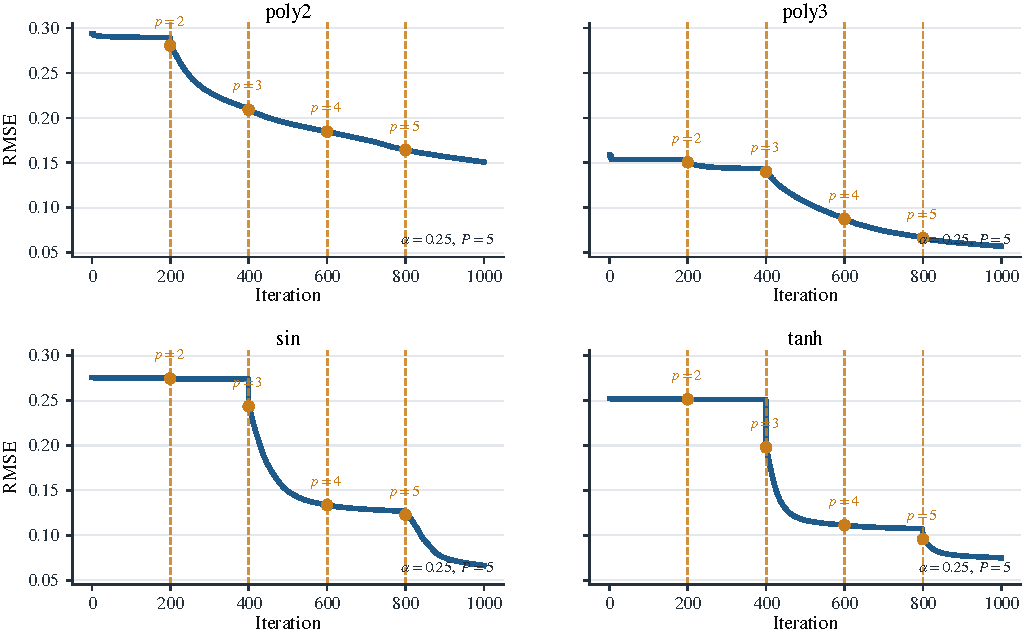
\includegraphics[width=\textwidth]{./inputs/figures/main/nonlinear_step_grid.pdf}
    \caption{Training-loss curves of NTD-PL under the progressive degree-increasing strategy.}
    \label{fig:rmse_step_grid}
\end{figure}

\subsection{Nonlinear Low-Rank Reconstruction and Completion on Hyperspectral Data}
\label{sec:real_hsi_representation}

We now turn to experimental validation on real hyperspectral data. We focus on answering three questions. First, does the overall gain of NTD-PL over linear Tucker still hold in real scenes? Second, where exactly does this gain come from? Third, does this advantage exhibit clear spatial localization, degree-related mechanisms, and cross-dataset stability? To answer these questions, the remainder of this section proceeds through six aspects: full-observation reconstruction, random-missing completion, mechanism discrimination, localization of local gains, analysis of degree saturation, and cross-dataset robustness, thereby forming a complete chain of evidence from overall performance to mechanism interpretation to external validation.

\subsubsection{Data and Protocol}

The experiments are organized into two layers: primary mechanism analysis and external robustness validation. The main experiments use $15$ scenes from the CAVE dataset \cite{cave_multispectral_database,yasuma2010gapc} to systematically analyze the overall gains of NTD-PL on real hyperspectral tensors, the spatial distribution of local gains, and the mechanism related to polynomial degree. The external validation further uses four commonly used benchmark scenes, Jasper Ridge \cite{roberts1993jasperridge}, Samson \cite{davis2007samson}, Urban \cite{urban_hypercube_dataset}, and Cuprite \cite{resmini1997cuprite}, to test whether the main conclusions continue to hold across different spatial sizes, numbers of spectral bands, and scene properties.

All real-data experiments are conducted under full observation, with the original data size preserved, no additional cropping or downsampling, and no special selection of particular scenes. In preprocessing, we uniformly use global max normalization. The evaluation metrics follow Section~\ref{sec:exp-setup}: full-observation reconstruction reports RMSE, NMSE(dB), and SAM; random-missing completion uses RMSE$^\ast$, NMSE(dB)$^\ast$, and SAM$^\ast$, computed only on the missing entries, as the main metrics. For the completion experiments, Tucker and NTD-PL share the same observation mask under the same scene, missing rate, and random seed, so as to ensure a fair paired comparison.

For parameters, the main text reports three rank budgets for CAVE full-observation reconstruction, namely $(24,24,4)$, $(33,33,4)$, and $(40,40,5)$, in order to examine whether the trend remains stable under different compression levels. For CAVE random-missing completion, we uniformly consider four missing rates, $\rho=0.1,0.3,0.5,0.7$, and compare Tucker and NTD-PL under the same rank setting and the same training protocol. The later mechanism comparison, hard-pixel / boundary-region analysis, and degree-mechanism analysis are all built on this unified completion protocol, so as to avoid introducing additional confounding factors through changes in task setup.

The cross-dataset robustness validation no longer uses one fixed rank. Instead, for each dataset, a rank setting is automatically determined by a unified compression-ratio matching rule. For these additional datasets, the completion task uniformly uses a random element-wise missing rate of $\rho=0.5$. Therefore, the cross-dataset comparison in the main text is not based on individually tuned best-case results for each dataset, but is an external validity test across different real scenes under a unified protocol.

\subsubsection{Full-Observation Reconstruction}

We first examine low-rank reconstruction performance under full observation. Table~\ref{tab:cave_recon} reports the scene-wise mean results under the three parameter budgets. It can be seen that under all three settings, $(24,24,4)$, $(33,33,4)$, and $(40,40,5)$, NTD-PL achieves lower RMSE, lower NMSE(dB), and lower SAM than Tucker. This shows that polynomial links bring stable gains while keeping the parameter scale of the Tucker low-rank backbone unchanged.

\begin{table}[htbp]
    \centering
    \caption{Full-observation low-rank reconstruction results on CAVE. Under all three rank settings, NTD-PL and Tucker are compared under the same parameter budget, and NTD-PL achieves lower RMSE, NMSE(dB), and SAM.}
    \label{tab:cave_recon}
    \small
    \begin{tabular}{@{}c l r c c c@{}}
\toprule
Rank & Method & Param. & RMSE$\downarrow$ & NMSE(dB)$\downarrow$ & SAM($^\circ$)$\downarrow$\\
\midrule
\multirow{2}{*}{$(24, 24, 4)$} & Tucker & 27,004 & 0.0299 $\pm$ 0.0198 & -17.610 $\pm$ 4.498 & 17.42 $\pm$ 7.42 \\
 & NTD-PL & 27,011 & \textbf{0.0256 $\pm$ 0.0178} & \textbf{-19.058 $\pm$ 4.725} & \textbf{15.15 $\pm$ 6.40} \\
\midrule
\multirow{2}{*}{$(33, 33, 4)^{\star}$} & Tucker & 38,272 & 0.0261 $\pm$ 0.0172 & -18.801 $\pm$ 4.432 & 16.43 $\pm$ 7.22 \\
 & NTD-PL & 38,279 & \textbf{0.0223 $\pm$ 0.0150} & \textbf{-20.125 $\pm$ 4.515} & \textbf{14.41 $\pm$ 6.30} \\
\midrule
\multirow{2}{*}{$(40, 40, 5)$} & Tucker & 49,115 & 0.0217 $\pm$ 0.0161 & -20.739 $\pm$ 5.089 & 12.65 $\pm$ 5.93 \\
 & NTD-PL & 49,122 & \textbf{0.0192 $\pm$ 0.0135} & \textbf{-21.509 $\pm$ 4.540} & \textbf{11.85 $\pm$ 5.84} \\
\midrule
\multicolumn{6}{l}{\footnotesize $\star$ Main report rank in Sec.~5.3.2.}\\
\bottomrule
\end{tabular}

\end{table}

\begin{table}[htbp]
    \centering
    \caption{Scene-level comparison for full-observation reconstruction on CAVE. NTD-PL outperforms Tucker on the vast majority of scenes, indicating that the overall gain is not driven by only a few anomalous scenes.}
    \label{tab:cave_recon_significance}
    \small
    \begin{tabular}{c c c c c}
\toprule
Metric & Win/Loss/Tie & Median gain & Sign test $p$ & Wilcoxon $p$ \\
\midrule
RMSE & 14/1/0 & 0.0028 & $9.77 \times 10^{-4}$ & $1.22 \times 10^{-4}$ \\
NMSE\_dB & 14/1/0 & 1.1727 & $9.77 \times 10^{-4}$ & $1.22 \times 10^{-4}$ \\
SAM & 13/2/0 & 1.6423 & 0.007 & 0.022 \\
\bottomrule
\end{tabular}

\end{table}

\begin{figure}[htbp]
    \centering
    
\includegraphics[width=\linewidth]{./inputs/figures/main/cave_reconstruction_scene_gain.pdf}
    \caption{Scene-level visualization of full-observation reconstruction on CAVE. Each line connects the Tucker and NTD-PL results for the same scene. Overall, most scenes shift toward the side where NTD-PL is better, indicating consistency of the advantage at the scene level.}
    \label{fig:cave_scene_improvement}
\end{figure}

\begin{figure}[htbp]
    \centering
    
\includegraphics[width=\textwidth]{./inputs/figures/main/cave_reconstruction_visual_grid.pdf}
    \caption{Spatial visualization of full-observation reconstruction on CAVE. Each row corresponds to a representative scene and shows the original image, reconstruction, pixel-wise error map, and error-reduction map. In the last column, positive values indicate that NTD-PL further reduces the reconstruction error relative to Tucker.}
    \label{fig:cave_full_visual}
\end{figure}

\begin{figure}[htbp]
    \centering
    
\includegraphics[width=\textwidth]{./inputs/figures/main/cave_reconstruction_spectra.pdf}
    \caption{Representative spectral-line comparison for full-observation reconstruction on CAVE. The figure shows the ground-truth and reconstructed spectra for the corresponding pixels. The annotated $\Delta$RMSE and $\Delta$SAM indicate the improvements relative to Tucker.}
    \label{fig:cave_full_spectral}
\end{figure}

\subsubsection{Random-Observation Completion}

Under random missing observations, we further examine the behavior of NTD-PL in recovering missing entries. Table~\ref{tab:cave_random_completion} gives the main results under four missing rates. It can be seen that under all settings, $\rho=0.1,0.3,0.5,0.7$, NTD-PL consistently outperforms Tucker, with clear improvements in both RMSE$^\ast$ and SAM$^\ast$. This indicates that the advantage of NTD-PL is not limited to mild correction at low missing rates, but remains stable from mild to severe missingness. In particular, at the highest missing rate, $\rho=0.7$, the improvement in RMSE$^\ast$ becomes even larger, suggesting that when available observations are sparser, nonlinearity still plays a clear role in recovering missing entries.

\begin{table}[htbp]
    \centering
    \caption{Main results for random-missing completion on CAVE. Under all four missing rates, NTD-PL outperforms Tucker, showing that the gain directly manifests in the recovery quality at the missing entries.}
    \label{tab:cave_random_completion}
    \small
    \begin{tabular}{c l c c c}
    \toprule
    $\rho$ & Method & RMSE* & NMSE(dB)* & SAM* \\
    \midrule
    0.1 & Tucker & 0.0263 $\pm$ 0.0179 & -18.728 $\pm$ 4.581 & 11.82 $\pm$ 5.33 \\
     & NTD-PL & \textbf{0.0229 $\pm$ 0.0158} & \textbf{-19.909 $\pm$ 4.683} & \textbf{8.36 $\pm$ 3.38} \\
    \midrule
    0.3 & Tucker & 0.0263 $\pm$ 0.0179 & -18.707 $\pm$ 4.575 & 14.75 $\pm$ 6.33 \\
     & NTD-PL & \textbf{0.0230 $\pm$ 0.0158} & \textbf{-19.864 $\pm$ 4.664} & \textbf{12.47 $\pm$ 5.06} \\
    \midrule
    0.5 & Tucker & 0.0264 $\pm$ 0.0179 & -18.688 $\pm$ 4.582 & 15.56 $\pm$ 6.85 \\
     & NTD-PL & \textbf{0.0230 $\pm$ 0.0158} & \textbf{-19.865 $\pm$ 4.691} & \textbf{13.48 $\pm$ 5.75} \\
    \midrule
    0.7 & Tucker & 0.0266 $\pm$ 0.0180 & -18.614 $\pm$ 4.573 & 16.02 $\pm$ 7.21 \\
     & NTD-PL & \textbf{0.0219 $\pm$ 0.0128} & \textbf{-20.043 $\pm$ 4.227} & \textbf{13.79 $\pm$ 5.43} \\
    \bottomrule
\end{tabular}

\end{table}

\begin{table}[htbp]
    \centering
    \caption{Scene-level comparison for random-missing completion on CAVE. Under all missing rates, the difference is uniformly defined as Tucker $-$ NTD-PL, so positive values indicate that NTD-PL is better. The results show that the completion gain is significantly consistent at the scene level across different missing rates.}
    \label{tab:cave_completion_significance}
    \small
    \begin{tabular}{c c c c c c}
\toprule
$\rho$ & Metric & Win/Loss/Tie & Median gain & Sign test $p$ & Wilcoxon $p$ \\
\midrule
0.1 & RMSE* & 14/1/0 & 0.0027 & 9.77$\times 10^{-4}$ & 1.22$\times 10^{-4}$ \\
0.1 & SAM* & 14/1/0 & 2.9742 & 9.77$\times 10^{-4}$ & 8.54$\times 10^{-4}$ \\
0.3 & RMSE* & 14/1/0 & 0.0027 & 9.77$\times 10^{-4}$ & 1.22$\times 10^{-4}$ \\
0.3 & SAM* & 13/2/0 & 1.9194 & 0.007 & 0.004 \\
0.5 & RMSE* & 14/1/0 & 0.0026 & 9.77$\times 10^{-4}$ & 1.22$\times 10^{-4}$ \\
0.5 & SAM* & 13/2/0 & 1.6566 & 0.007 & 0.012 \\
0.7 & RMSE* & 14/1/0 & 0.0027 & 9.77$\times 10^{-4}$ & 1.22$\times 10^{-4}$ \\
0.7 & SAM* & 12/3/0 & 1.3394 & 0.035 & 0.048 \\
\bottomrule
\end{tabular}

\end{table}

\subsubsection{Mechanism Distinction from Polynomial Post-Processing}

The previous two subsections have shown that NTD-PL consistently outperforms Tucker in both full-observation reconstruction and random-missing completion. However, one question still needs to be answered more carefully: where exactly does this gain come from? One possible explanation is that the advantage of NTD-PL may not require joint modeling at all; perhaps one could simply obtain a Tucker reconstruction first and then apply an element-wise polynomial calibration to its output. To distinguish between these possibilities, we introduce a post-processing baseline, \emph{PolyCal}. This method first trains standard Tucker, and then fits a shared element-wise fourth-order polynomial response mapping on its output, thereby post-correcting the entry-level response without changing the low-rank backbone.

\begin{table}[htbp]
    \centering
    \caption{Main table for the mechanism comparison. The three methods are compared on full-observation reconstruction and random-missing completion at $\rho=0.5$. PolyCal applies a shared element-wise polynomial calibration after Tucker output, whereas NTD-PL jointly models the nonlinear link and the low-rank backbone.}
    \label{tab:mechanism_closure}
    \small
    \begin{tabular}{@{}c l r c c@{}}
\toprule
Setting & Method & Param. & RMSE$\downarrow$ & SAM$\downarrow$ \\
\midrule
    \multirow{3}{*}{Recon.} & Tucker & 38,272 & 0.02606 $\pm$ 0.01718 & 16.4329 $\pm$ 7.2207 \\
     & PolyCal & 38,277 & 0.02557 $\pm$ 0.01661 & 15.4054 $\pm$ 6.3013 \\
     & NTD-PL & 38,279 & \textbf{0.02234 $\pm$ 0.01497} & \textbf{14.4082 $\pm$ 6.3010} \\
    \midrule
    \multirow{3}{*}{Compl.} & Tucker & 38,272 & 0.02637 $\pm$ 0.01791 & 15.5569 $\pm$ 6.8502 \\
     & PolyCal & 38,277 & 0.02587 $\pm$ 0.01731 & 14.3420 $\pm$ 5.7617 \\
     & NTD-PL & 38,277 & \textbf{0.02299 $\pm$ 0.01582} & \textbf{13.4841 $\pm$ 5.7459} \\
\bottomrule
\end{tabular}

\end{table}

\begin{figure}[htbp]
    \centering
    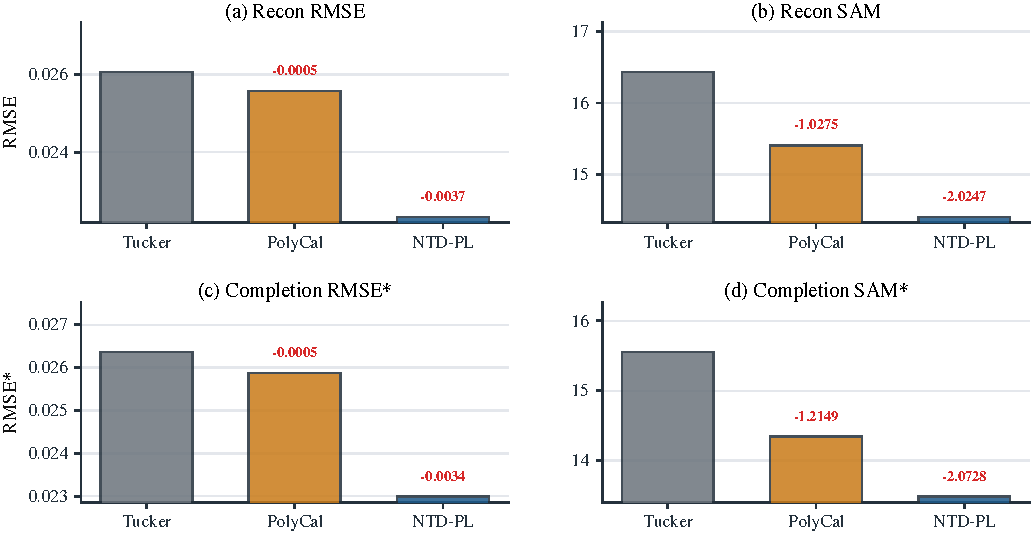
\includegraphics[width=\textwidth]{./inputs/figures/main/mechanism_closure_main_figure.pdf}
    \caption{Main figure for mechanism discrimination. The four panels compare RMSE and SAM for full-observation reconstruction, and RMSE$^\ast$ and SAM$^\ast$ for completion at $\rho=0.5$. All three methods exhibit a consistent improvement relationship, showing that post-processing can only partially approach the gains of NTD-PL and cannot replace its joint modeling.}
    \label{fig:mechanism_closure_main}
\end{figure}

\subsubsection{Where the Advantage Appears}

This subsection focuses on a more specific question: where exactly in the image does the additional gain of NTD-PL occur? If its effect were merely a globally smooth correction, the gain should be approximately uniform. If, instead, it corrects the local structures that are hardest for linear low-rank models to fit, the gain should concentrate near difficult regions and structural boundaries.

\begin{figure}[htbp]
    \centering
    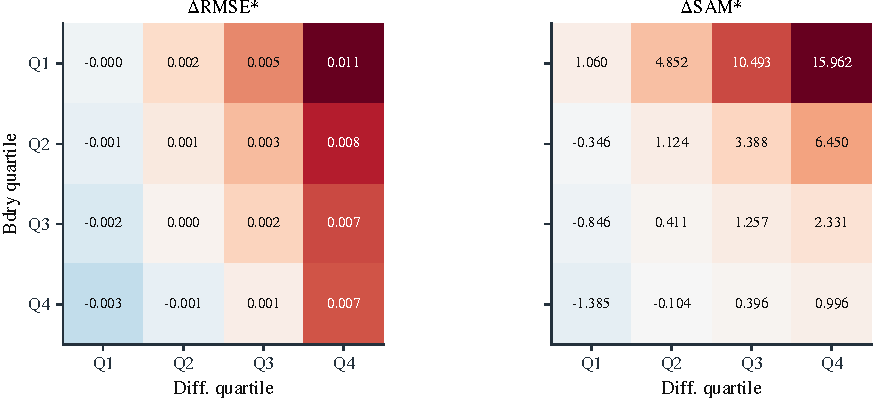
\includegraphics[width=\textwidth]{./inputs/figures/main/cave_completion_advantage_heatmap.pdf}
    \caption{Two-dimensional distribution of the local gain of NTD-PL over Tucker across difficulty quartiles and boundary quartiles. Positive values indicate that NTD-PL is better. One can see that the gain is not uniformly distributed, but is concentrated mainly in the intersection of difficult and boundary-rich regions.}
    \label{fig:cave_completion_advantage_heatmap}
\end{figure}

\begin{figure}[htbp]
    \centering
    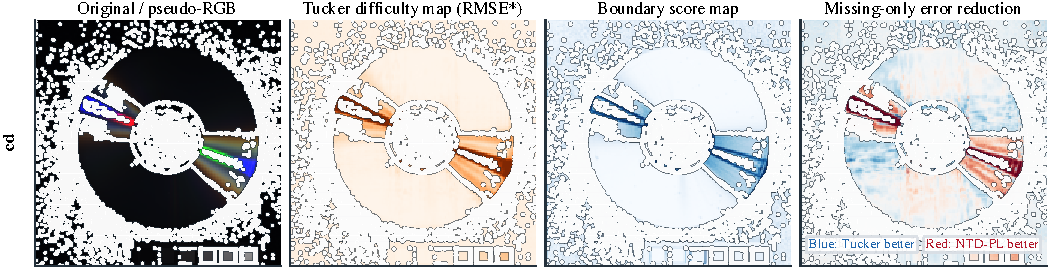
\includegraphics[width=\textwidth]{./inputs/figures/main/cave_completion_advantage_spatial_case.pdf}
    \caption{Localization of local gain on the representative \texttt{cd} scene. The four columns show, in order, the pseudo-RGB original image, the difficulty map (brighter orange indicates greater difficulty), the boundary map (brighter blue indicates stronger boundaries), and the missing-only error reduction map (red indicates NTD-PL is better and blue indicates Tucker is better). The white contour marks the intersection of the top-difficulty and top-boundary regions. One can see that the positive gain is concentrated mainly at locations where high difficulty and strong boundaries occur simultaneously.}
    \label{fig:cave_completion_advantage_spatial}
\end{figure}

\subsubsection{Examination of the Polynomial Degree}

To examine which orders provide the main gains in NTD-PL, we scan the maximum polynomial degree $P$ under the same CAVE random-missing completion setting as above, and record both the missing-only metrics and the effective contribution of each degree term. The left panel of Figure~\ref{fig:parameter_mechanism} shows that completion performance continues to improve as $P$ increases from $1$ to $4$, but the main gains are concentrated in the low- to medium-order range, and the benefit from further increasing the degree becomes clearly weaker. The right panel further shows that the model contribution is mainly carried by the second- and third-order terms: once $P\ge 3$, these two terms remain dominant, while the fourth-order term contributes only a small marginal correction. This indicates that the main mismatch in real hyperspectral completion does not require very high-order degrees of freedom to describe; explicit nonlinearity of low to medium order is already sufficient to absorb most of the nonlinear residual.

\begin{figure}[htbp]
    \centering
    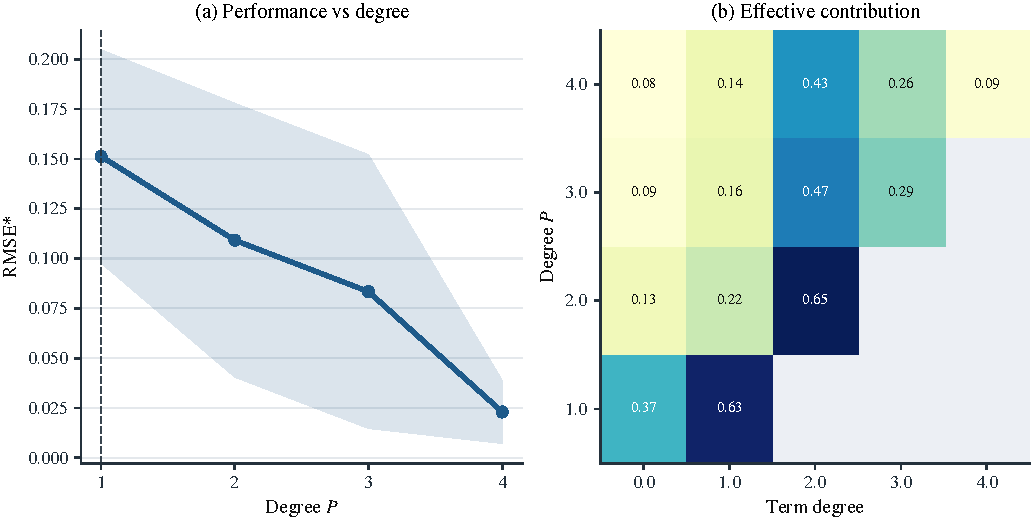
\includegraphics[width=\linewidth]{./inputs/figures/main/cave_parameter_mechanism.pdf}
    \caption{Degree-mechanism analysis for random-missing completion on CAVE. The left panel shows the main missing-entry metrics as a function of the maximum polynomial degree $P$; the right panel shows the average effective contribution of each degree term under different $P$.}
    \label{fig:parameter_mechanism}
\end{figure}

\subsubsection{Cross-Dataset Robustness Validation}

To test whether the above conclusions hold only on CAVE, we further conduct external validation on Jasper Ridge, Samson, Urban, and Cuprite, considering both full-observation reconstruction and random-missing completion. All datasets use full-scene settings, global max normalization, and ranks automatically determined by the same compression-ratio matching rule. The completion task uniformly uses a random element-wise missing rate of $\rho=0.5$. Table~\ref{tab:real_hsi_robustness} shows that the advantage of NTD-PL is not CAVE-specific. On Jasper Ridge, Samson, and Urban, NTD-PL outperforms Tucker in both reconstruction and completion, and $\Delta$NMSE(dB) and $\Delta$SAM mostly improve in the same direction. Overall, under the RMSE metric, $7$ out of $8$ dataset $\times$ task combinations show positive gains, indicating that the advantage is fairly stable across different scenes and tasks. Cuprite, however, provides a clear boundary case: on this scene, the gains of NTD-PL are substantially weaker, and Tucker is slightly better on some metrics. This indicates that when the data are closer to classical linear mixing and the entry-level nonlinear deviation is weaker, Tucker can already explain the main structure well, and polynomial links can then bring only limited marginal improvement. Therefore, the conclusion about NTD-PL should be understood as follows: it can stably improve Tucker in most real hyperspectral scenes, but this advantage is not unconditional; its effectiveness still depends on the strength of the entry-level nonlinear residual in the data.

\begin{table}[htbp]
    \centering
    \caption{Main table for cross-dataset robustness validation. In the Recon. rows, Tucker / NTD-PL denotes RMSE; in the Compl. rows, Tucker / NTD-PL denotes RMSE$^\ast$. Gain(\%), $\Delta$NMSE(dB), and $\Delta$SAM are uniformly defined as Tucker $-$ NTD-PL, so positive values indicate that NTD-PL is better.}
    \label{tab:real_hsi_robustness}
    \small
    \begin{tabular}{@{}l l c c c c c c@{}}
    \toprule
    Dataset & Task & Rank & Tucker & NTD-PL & Gain(\%) & $\Delta$NMSE(dB) & $\Delta$SAM($^\circ$) \\
    \midrule
    Jasper Ridge & Recon. & (11,11,43) & 0.04623 & 0.04302 & \textbf{6.93} & \textbf{0.623} & \textbf{0.981} \\
     & Compl. & (11,11,43) & 0.04710 & 0.04342 & \textbf{7.82} & \textbf{0.708} & \textbf{1.156} \\
    \midrule
    Samson & Recon. & (10,10,35) & 0.02626 & 0.02417 & \textbf{7.95} & \textbf{0.719} & \textbf{0.057} \\
     & Compl. & (10,10,35) & 0.02681 & 0.02444 & \textbf{8.86} & \textbf{0.806} & \textbf{0.310} \\
    \midrule
    Urban & Recon. & (43,43,47) & 0.04444 & 0.04285 & \textbf{3.59} & \textbf{0.318} & \textbf{0.288} \\
     & Compl. & (43,43,47) & 0.04538 & 0.04326 & \textbf{4.67} & \textbf{0.415} & \textbf{0.488} \\
    \midrule
    Cuprite & Recon. & (35,26,54) & 0.01759 & 0.01770 & -0.60 & -0.052 & -0.037 \\
     & Compl. & (35,26,54) & 0.01791 & 0.01781 & \textbf{0.56} & \textbf{0.048} & -0.004 \\
    \bottomrule
\end{tabular}

\end{table}
